% !TEX TS-program = pdflatex
% !TEX encoding = UTF-8 Unicode

\chapter{Classification and Results} \label{chapter:results}

%\pagenumbering{arabic}

\section{Problem Formulation}

Now that the dataset is entirely prepared, it has to be decided which classifiers are going to be used, what problem of classification are they actually tackling and how can the results be interpreted. 

Firstly, it is important to understand what is it that it's going to be classified and how and if it can be extrapolated to the actual problem we are trying to solve. Our dataset is comprised of healthy people that make up the controls, and a group of \gls{T2D} affected people, amounting the cases. Furthermore, these two groups were not necessarily genotyped by the same methods, or even sequenced by the same machines. As expected, this may lead to bias between the groups, which makes their classification easier but wrong. However, during the previous phases, certain aspects and mechanisms were already employed to deal or verify this situation. Foremost, by the analysis of the quality of the dataset, it is assumed that most of the genotypes of cases are correctly made and accordant with the reference genome, such as the controls groups knowingly is. Even if some variants are incorrectly called in either group, ultimately these are aggregated with many other variants in an attempt to represent a whole gene. This not only reduces the bias or noise the final features will have by dissolving the variants, but also allows for a representation that is understandable when those same features require further investigation. 

One extra step employed to try and remove bias, was adding information of the biological context to the dataset. This was performed using the risk genes. By utilizing them, it is known beforehand that these do add up significant observable differences that are less likely to come from bias. When these were forcefully included in the dataset without any kind of filtering such as the one performed with $\chi^2$, they only made up 18 out of 138 genes, or 13\% of the genes. This number almost doubled when there was a search for the most important features, which found 24\% of the genes being already known as risk genes. This goes to show that the methods employed are indeed in the right track, and have a fair amount of success finding important and unbiased features.

Besides laying out the specific gene importance, that allows for follow up investigation on it, it is also possible to trace back the present variants on a single gene, and proceed with a closer inspection on specific \gls{SNP}s and their genotypes. This nonetheless, still leads to the question of which is the correct approach for the problem, and what is it important to extract. Is it better to look at regions, or single variants are enough to explain the problem? Being able to detect mutations is important because it offers clear and concrete proof of what are the mechanisms behind the disease, and give credibility to the solution for genomics experts. However, this is not always possible, and if whole regions offer better results without specific alleles information, is it worthwhile to use them? For these questions, this approach enables answers for both, which might be important to justify using whole genes information not losing focus of smaller variants. 

From the classification problem, it is expected to distinguish between groups of people with higher risk of \gls{T2D} and healthy, only making use of genotypes. However, to specify the problem as such, there are a few assumptions that are required. First, that the genetic code does not undergo many changes during a person's lifetime \cite{ali2013genetics} and that a member of the cases group has higher risk of developing \gls{T2D}. The first assumption is acceptable to make, but there is no certainty on the second one. Since there is no access to physiological data of each patient, there is no telling which environmental conditions each is exposed to, therefore no specific information about habits versus heritability. Two people exposed to the same environmental conditions can have different outcomes regarding \gls{T2D} because of genetics, but someone with lower risk can be affected by \gls{T2D} solely through very high sugar levels in the blood. It is not known for sure if there are specific cases where genetics played a bigger role, but it is assumed that overall, the cases group has a higher risk of being affected by \gls{T2D}. There is no specific interest in classifying \gls{T2D} using more patient's data, but it would be helpful in such cases to perform a distinction between higher genetic \gls{T2D} risk, and therefore improving the problem's approach.

Ultimately, the solution requires a classifier that is capable of looking for non-linear relations on the data. There are several available classifiers, but for this particular case Support Vector Machines and Decision Trees (more particularly Extra-Trees classifiers) were deemed appropriate. Both are well suited to look for non-linear associations and handle medium-sized datasets. Deep Learning was also considered, but it is a black box where little information can be extracted about the biological context of the problem, and there are not enough samples to improve its performance in a meaningful way.

\section{Classifier Optimization}

There are many kernels and parameters that are possible for the classifiers, making it necessary to optimize them for the present dataset. For the optimization, a set number of parameters is given, and the best classifier is chosen based on the combinations of different parameters and a scoring function. Since this dataset is not terribly unbalanced, the scores are based on prediction accuracy. If it were, it would not be advisable to use accuracy as such, since it could be very high even if it misclassified one entire class.

For the \gls{SVM}, the parameters provided are displayed on table \ref{tab:svm_params}. For each dataset, the optimized parameters will be different, which also happens when using only the top 50 discovered features, the whole dataset, or only features related to known risk genes. However, to standardize the process, only one final set of parameters that were the best overall for each dataset were chosen. 

The C parameter, as explained previously refers to the number of violations of boundaries allowed, the tol is the tolerance for the stopping criterion, gamma is the coefficient for the kernels "poly", and "sigmoid and the degree refers to the polynomial degrees for the "poly" kernel. The final optimized \gls{SVM} had a Gaussian Radial Basis Function for its kernel, a C of 0.75, tol of 0.001 and gamma set to "auto" that uses for it's value $ \frac{1}{Number\ of\ features}$. The Gaussian \gls{RBF} uses the following equation to compute the kernel: 

\begin{equation}
K(a, b) = exp(-\gamma \norm{a-b}^2) \\
\end{equation}

, where $a$ and $b$ are the original vectors. The number of parameters tested is not more extensive since this would be extremely slow, even with the choice of combination of parameters being randomized. 

\begin{table}[h]
	\begin{tabular}{|l|l|>{\centering}p{.9cm}|>{\centering}p{.9cm}|>{\centering}p{.9cm}|l|}
		\hline
		Parameters & Values                                   \\ \hline
		kernel    & {[}'linear', 'poly', 'rbf', 'sigmoid'{]} \\ \hline
		C         & {[}0.25, 0.4, 0.5, 0.55, 0.75, 1{]}      \\ \hline
		tol       & {[}1e-3, 1e-4, 1e-5{]}                   \\ \hline
		gamma     & {[}25, 50, 75, 100, 150, 'auto'{]}       \\ \hline
		degree    & {[}1, 2, 3, 5, 10{]}                     \\ \hline
	\end{tabular}\\ \vskip .5cm
	\caption{Parameters for the \gls{SVM} classifier that were tested to find the most optimized one. }
	\label{tab:svm_params}  
\end{table}

The Extra Trees classifier parameters are displayed on table \ref{tab:rf_params}, and are different that the ones used before. The n\_estimators refer to the number of trees in the forest and the criterion to the impurity evaluator. Other parameters refer to single tree characteristics like min\_samples\_leaf to the minimum number of samples needed to form a node, min\_samples\_split to the minimum number to split a node and max\_leaf\_nodes to the maximum number of nodes on the tree (mostly to save memory).

The optimized predictor used 50 trees with the 'gini' criterion, at least one sample per node, a minimum of four to split a node and twenty max nodes per tree. 

\begin{table}[h]
	\begin{tabular}{|l|l|>{\centering}p{.9cm}|>{\centering}p{.9cm}|>{\centering}p{.9cm}|l|}
		\hline
		Parameters          & Values                   \\ \hline
		n\_estimators       & {[}25, 50, 75, 100{]}    \\ \hline
		criterion           & {[}'entropy', 'gini'{]}  \\ \hline
		min\_samples\_leaf  & {[}1, 2, 3, 5, 10{]}     \\ \hline
		min\_samples\_split & {[}2, 4, 5, 8, 10{]}     \\ \hline
		max\_leaf\_nodes    & {[}2, 20, 50, 75, 100{]} \\ \hline
	\end{tabular}\\ \vskip .5cm
	\caption{Parameters for the Extra Trees classifier that were tested to find the most optimized one.}
	\label{tab:rf_params}  
\end{table}

\section{Metrics and Results}

After optimization of classifiers, it is necessary to employ validation techniques and extract meaningful metrics that allow for higher confidence in the results of the classifiers. Nevertheless, these new cases are still from the same original dataset, and likely will have the same bias and noise. Although the ultimate metric to evaluate generalization is actual classification and validation in more datasets of the same type, this is not always possible.

For this particular case, 5 fold cross-validation was used and since in this problem the dataset is not terribly unbalanced, the tests were evaluated with the accuracy and F1-Scores. Since the F1-Scores don't account for True Negatives, the \gls{ROC} curves were also observed to select the best model possible. The Machine Learning python package Scikit-Learn combines unnecessary thresholds, which make some plots seem like they have fewer thresholds computed. By combining all these metrics, it is possible to get a good idea of how the classifiers are performing.

Since every metric, validation and classifier is decided, the plan for testing can now be formulated. There are three different datasets whose characteristics were previously detailed in the last chapter. These are the full dataset with all the features extracted for the selected genes, the dataset that only contains features related to known risk genes and the last one with the top 50 selected features. The original variants dataset was not used since it overfits very badly. To verify the consistency of results, for each dataset, a hundred classifiers were ran with five fold cross-validation (either \gls{SVM} or Extra Trees), and their average values were computed. Their confidence intervals are not displayed since they are extremely small, because the predictors were very consistent. The metrics can be observed on figure \ref{fig:results} and the ROC curves on the following images.

\begin{figure}[h]
	\centering
	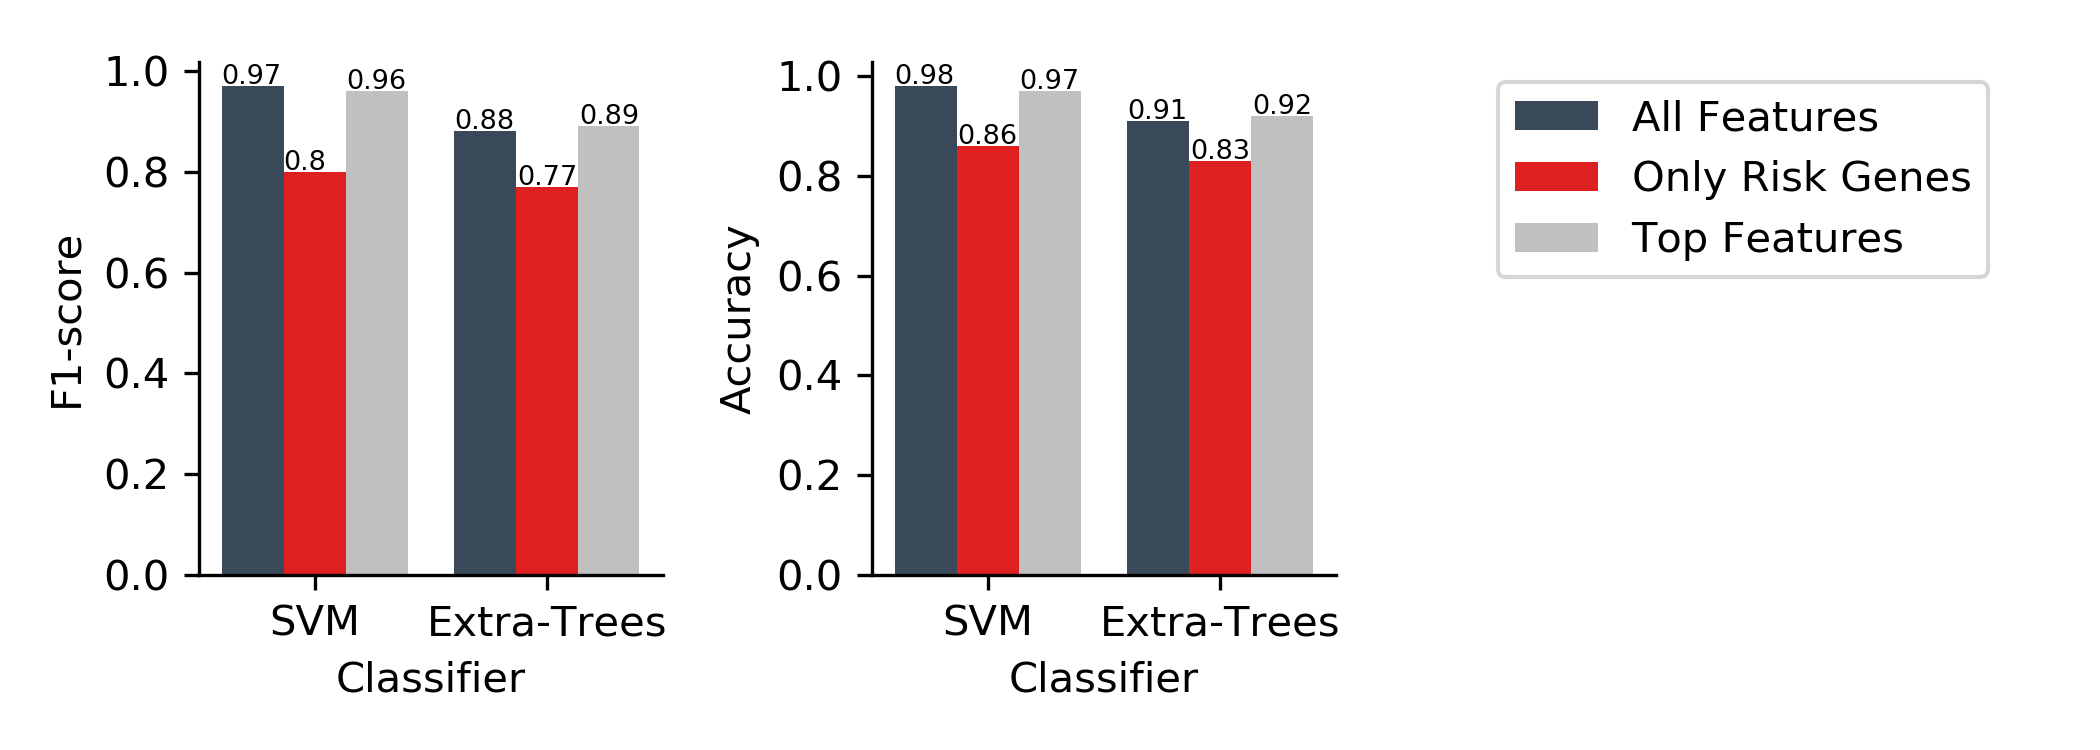
\includegraphics[width=\textwidth]{../images/results/class_results.png}
	\caption{Mean of F1-Scores and accuracies by classifier built with all the features (blue),
		only features from known risk genes (red) and top features identified in the previous
		analysis (silver). Results are the average of 100 trained classifiers for each situation.} 
	\label{fig:results}
\end{figure}

\newpage

\begin{figure}[H]
	\centering
	\includegraphics[width=5in]{../images/results/ET_all.png}
	\caption{ROC curve for the dataset with all features, with the Extra Trees Classifier.} 
	\label{fig:ET_all}
\end{figure}

\begin{figure}[H]
	\centering
	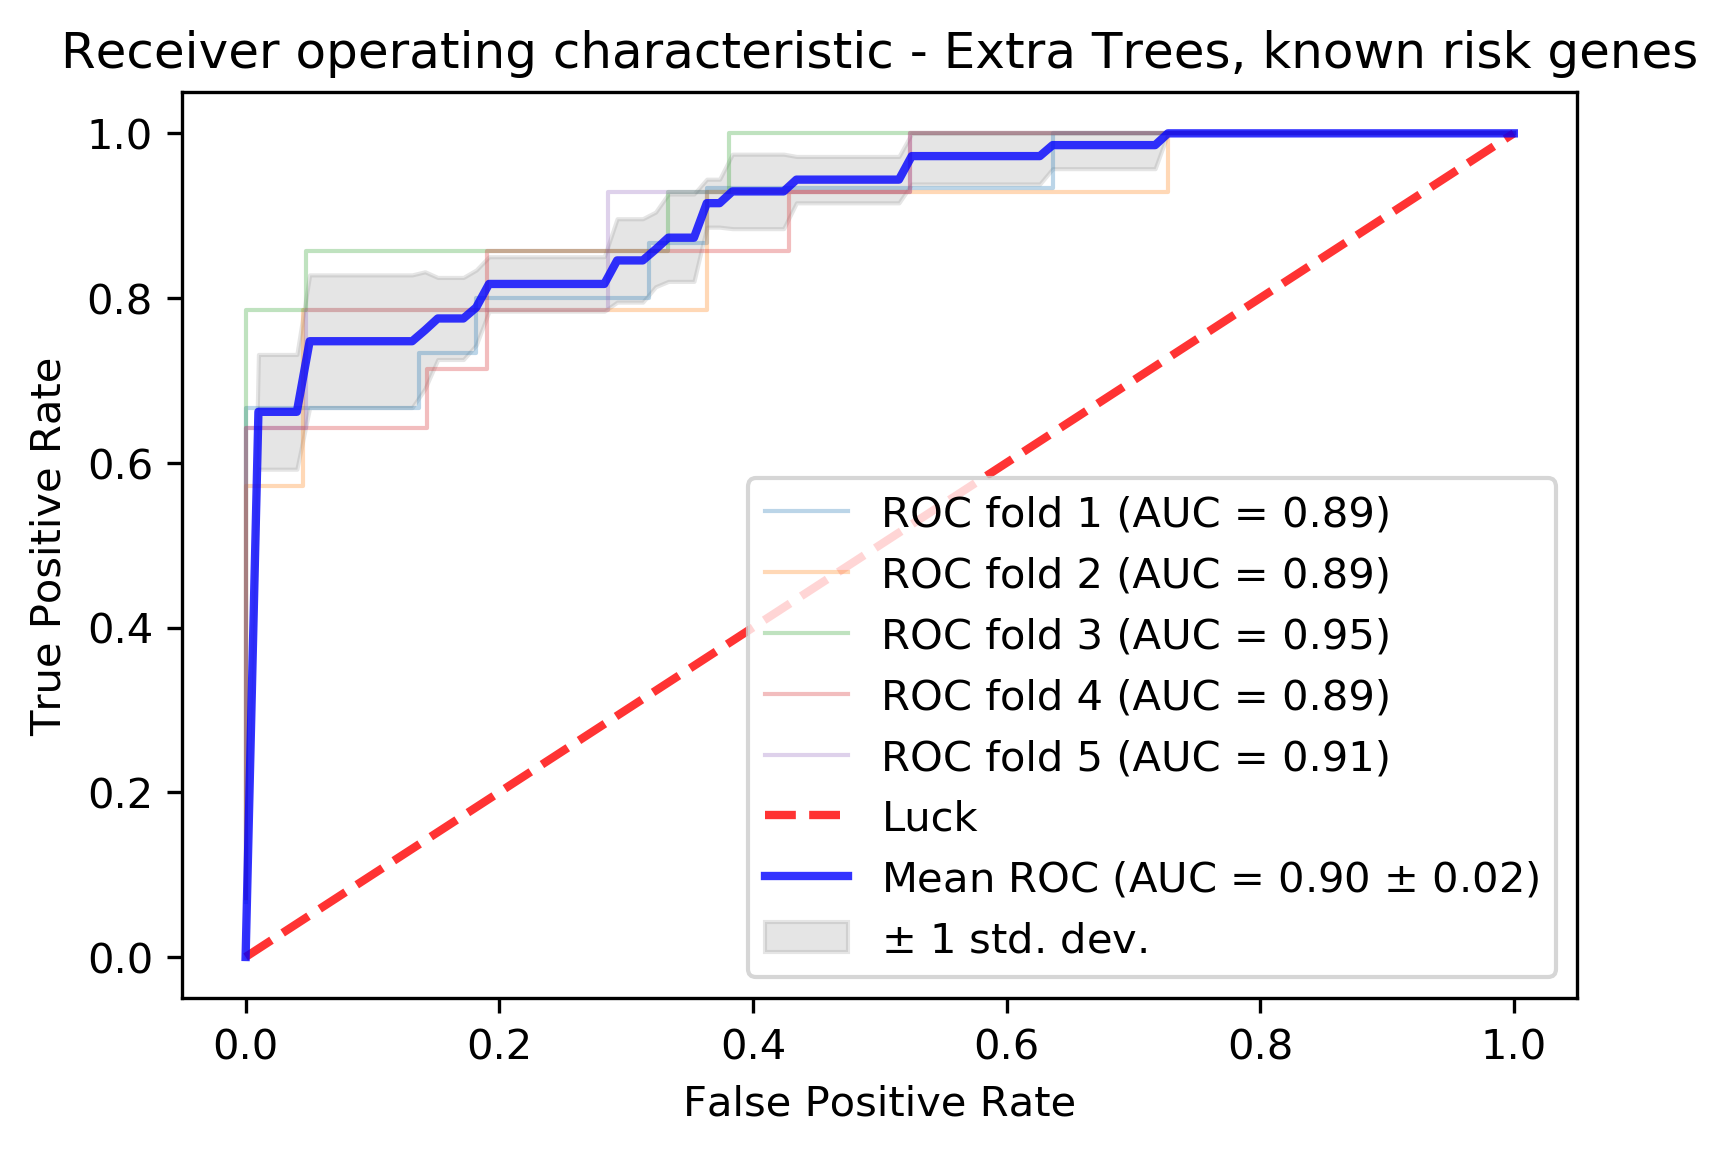
\includegraphics[width=5in]{../images/results/ET_risk.png}
	\caption{ROC curve for the dataset with the known risk genes features, with the Extra Trees Classifier.} 
	\label{fig:ET_risk}
\end{figure}


\begin{figure}[H]
	\centering
	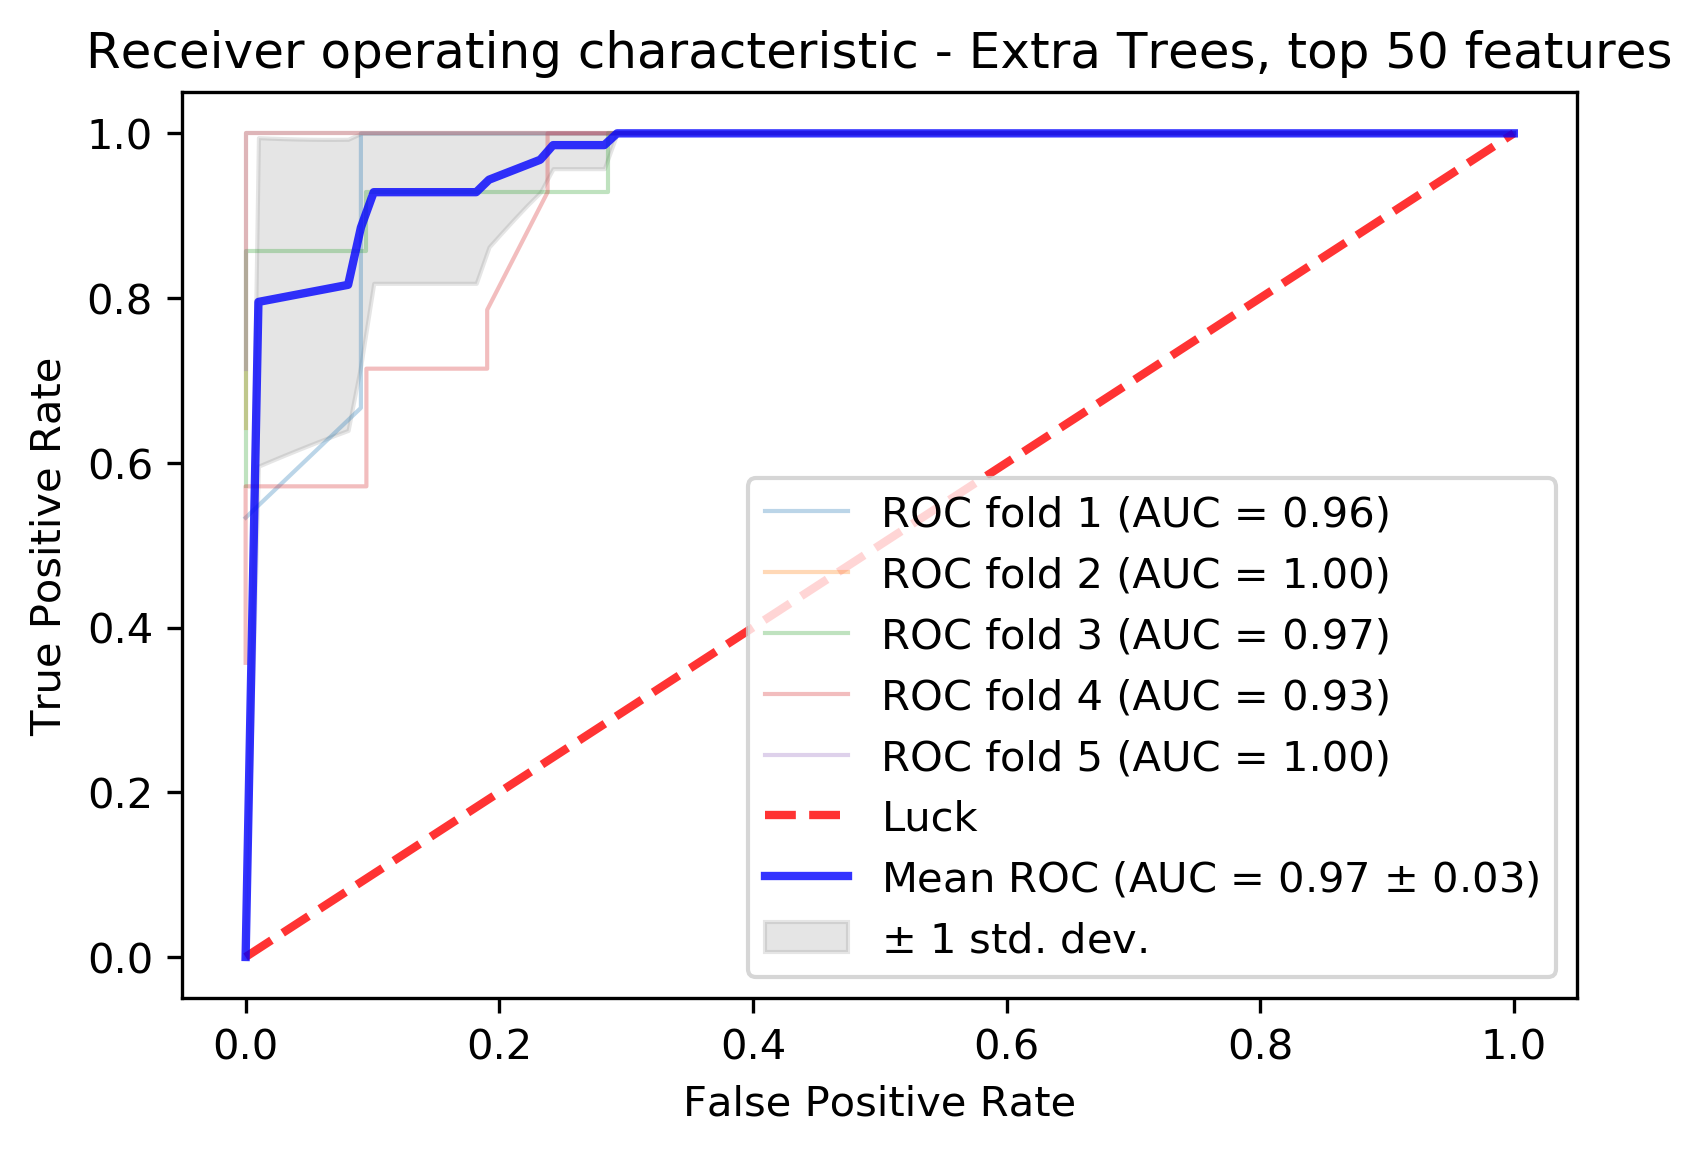
\includegraphics[width=5in]{../images/results/ET_top50.png}
	\caption{ROC curve for the dataset with the top fifty features, with the Extra Trees Classifier.} 
	\label{fig:ET_top}
\end{figure}

\begin{figure}[H]
	\centering
	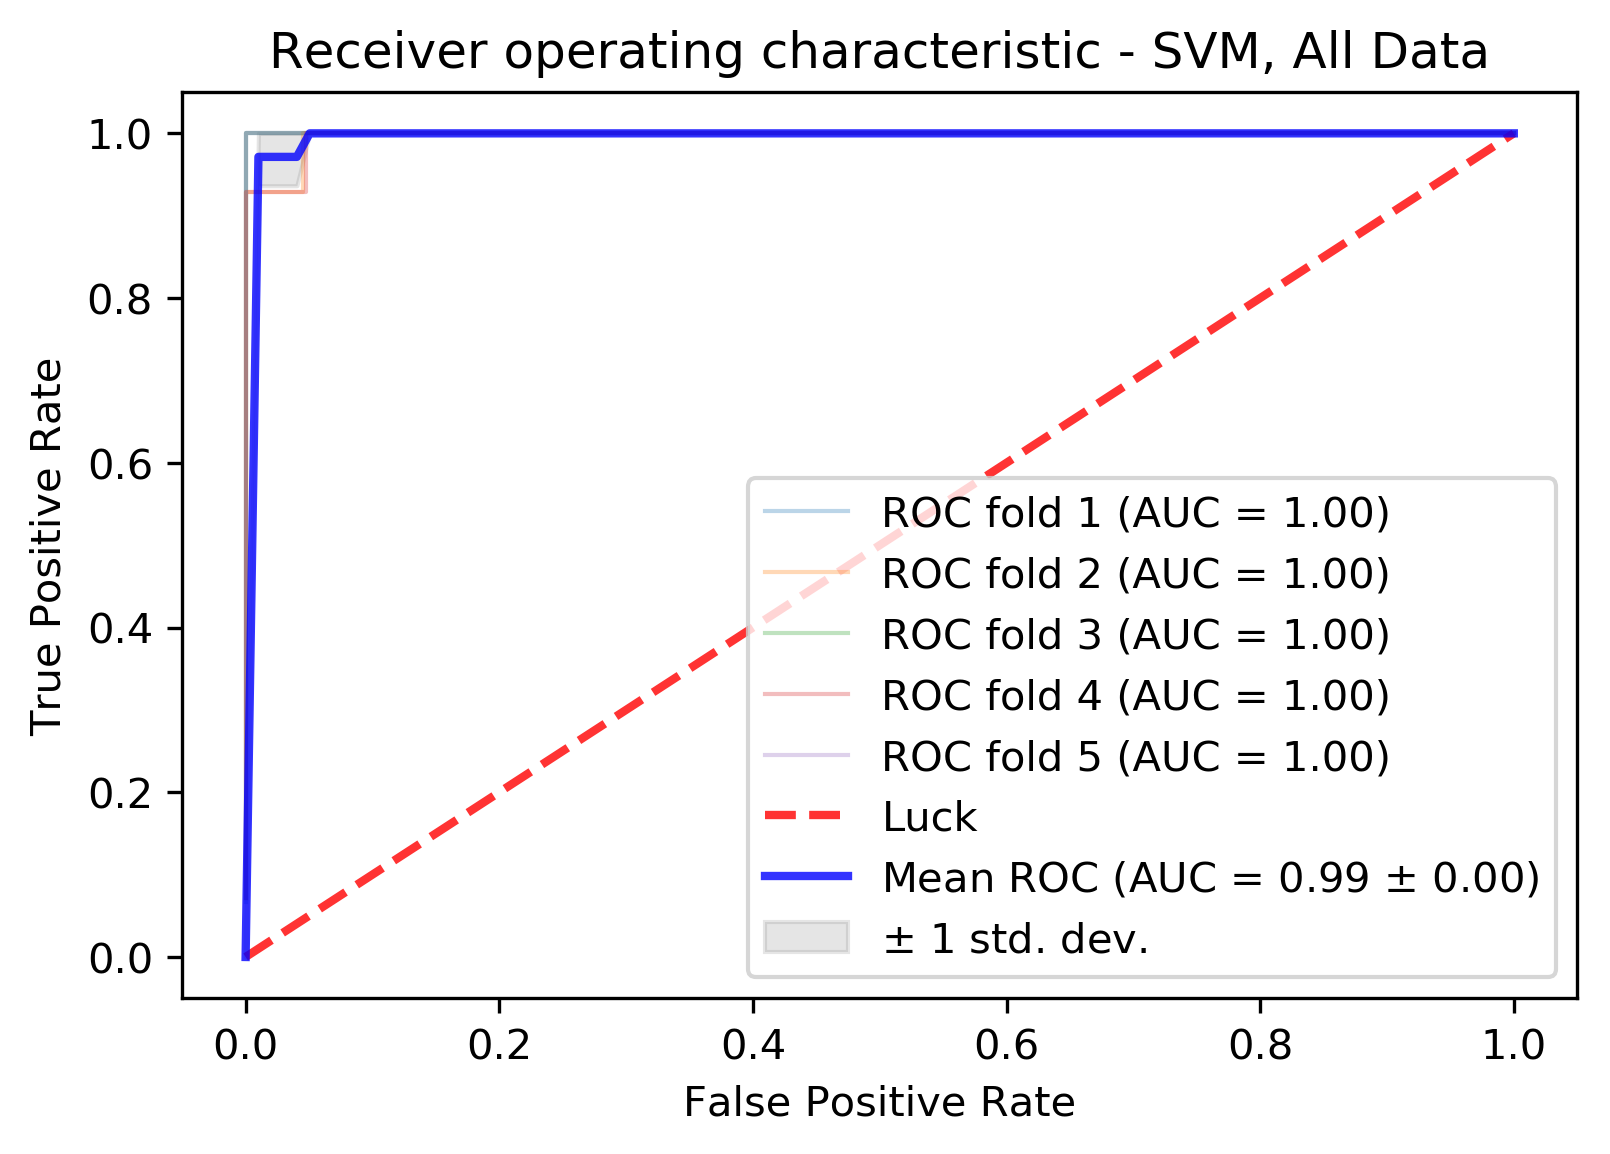
\includegraphics[width=5in]{../images/results/svm_all.png}
	\caption{ROC curve for the dataset with all features, with the SVM Classifier.} 
	\label{fig:svm_all}
\end{figure}

\begin{figure}[H]
	\centering
	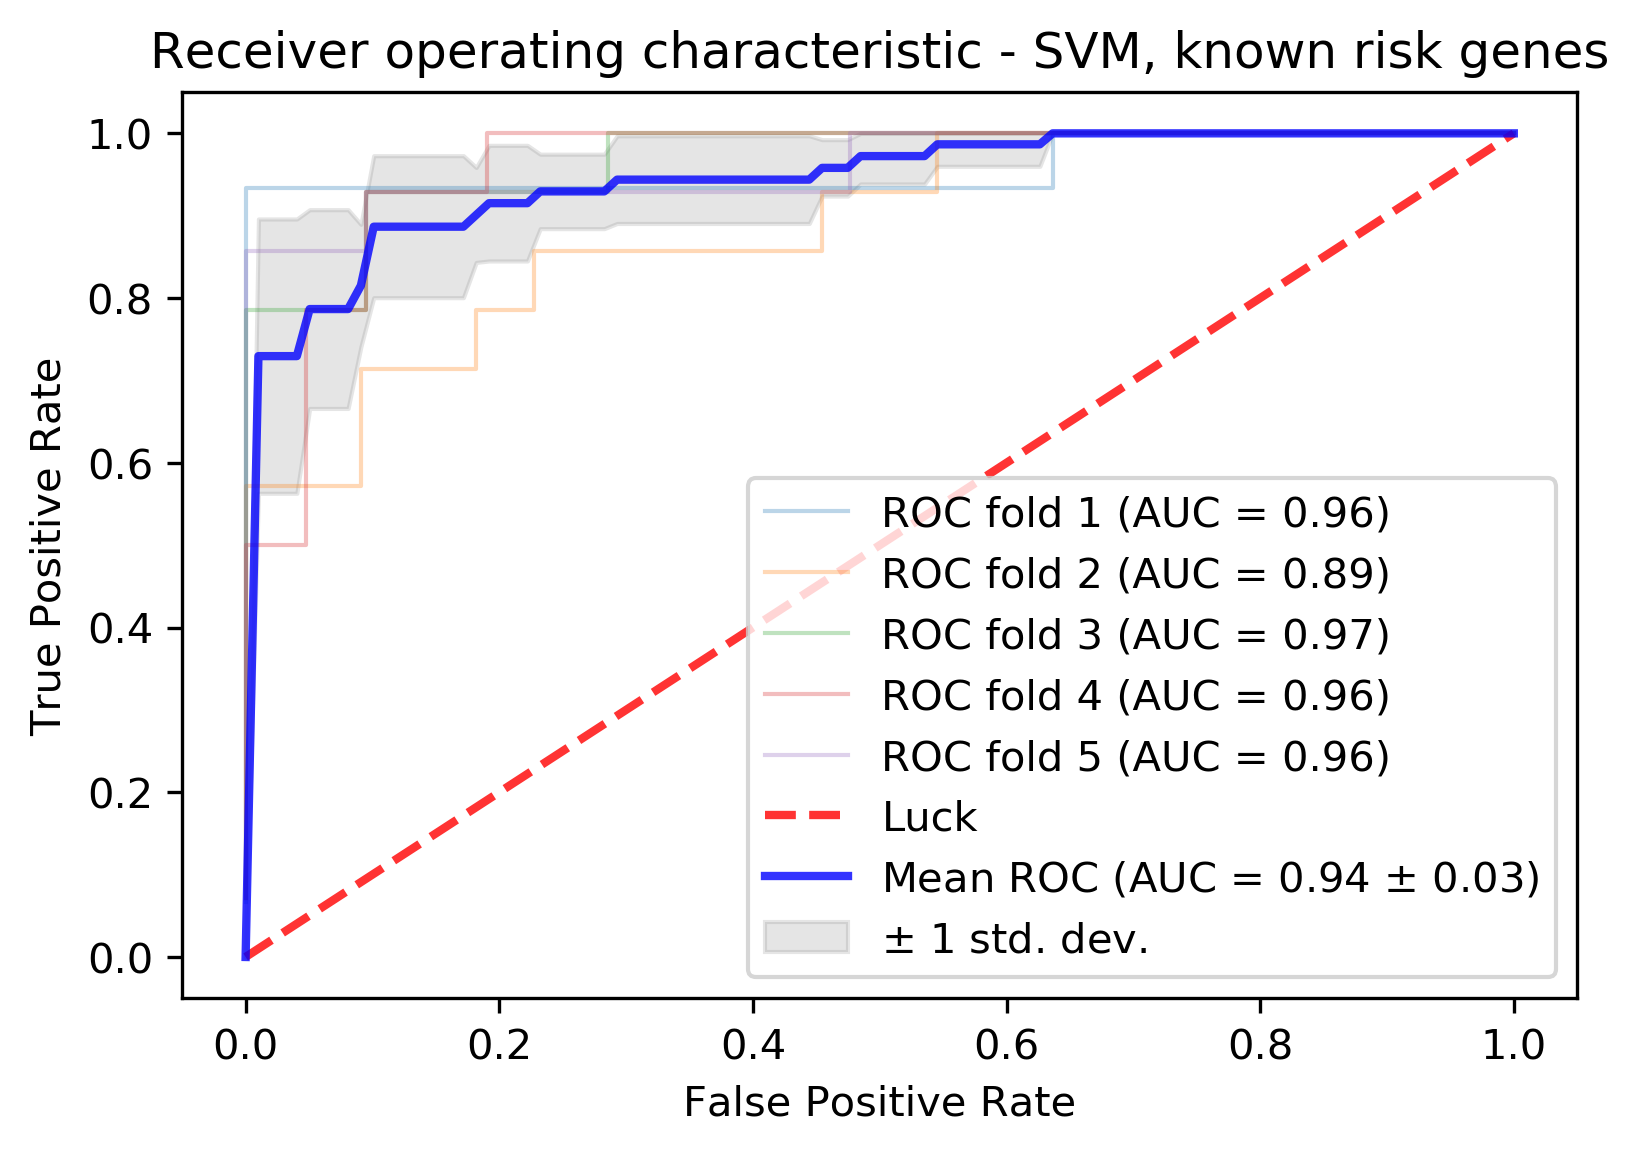
\includegraphics[width=5in]{../images/results/svm_risk.png}
	\caption{ROC curve for the dataset with the known risk genes features, with the SVM Classifier.} 
	\label{fig:svm_risk}
\end{figure}

\begin{figure}[H]
	\centering
	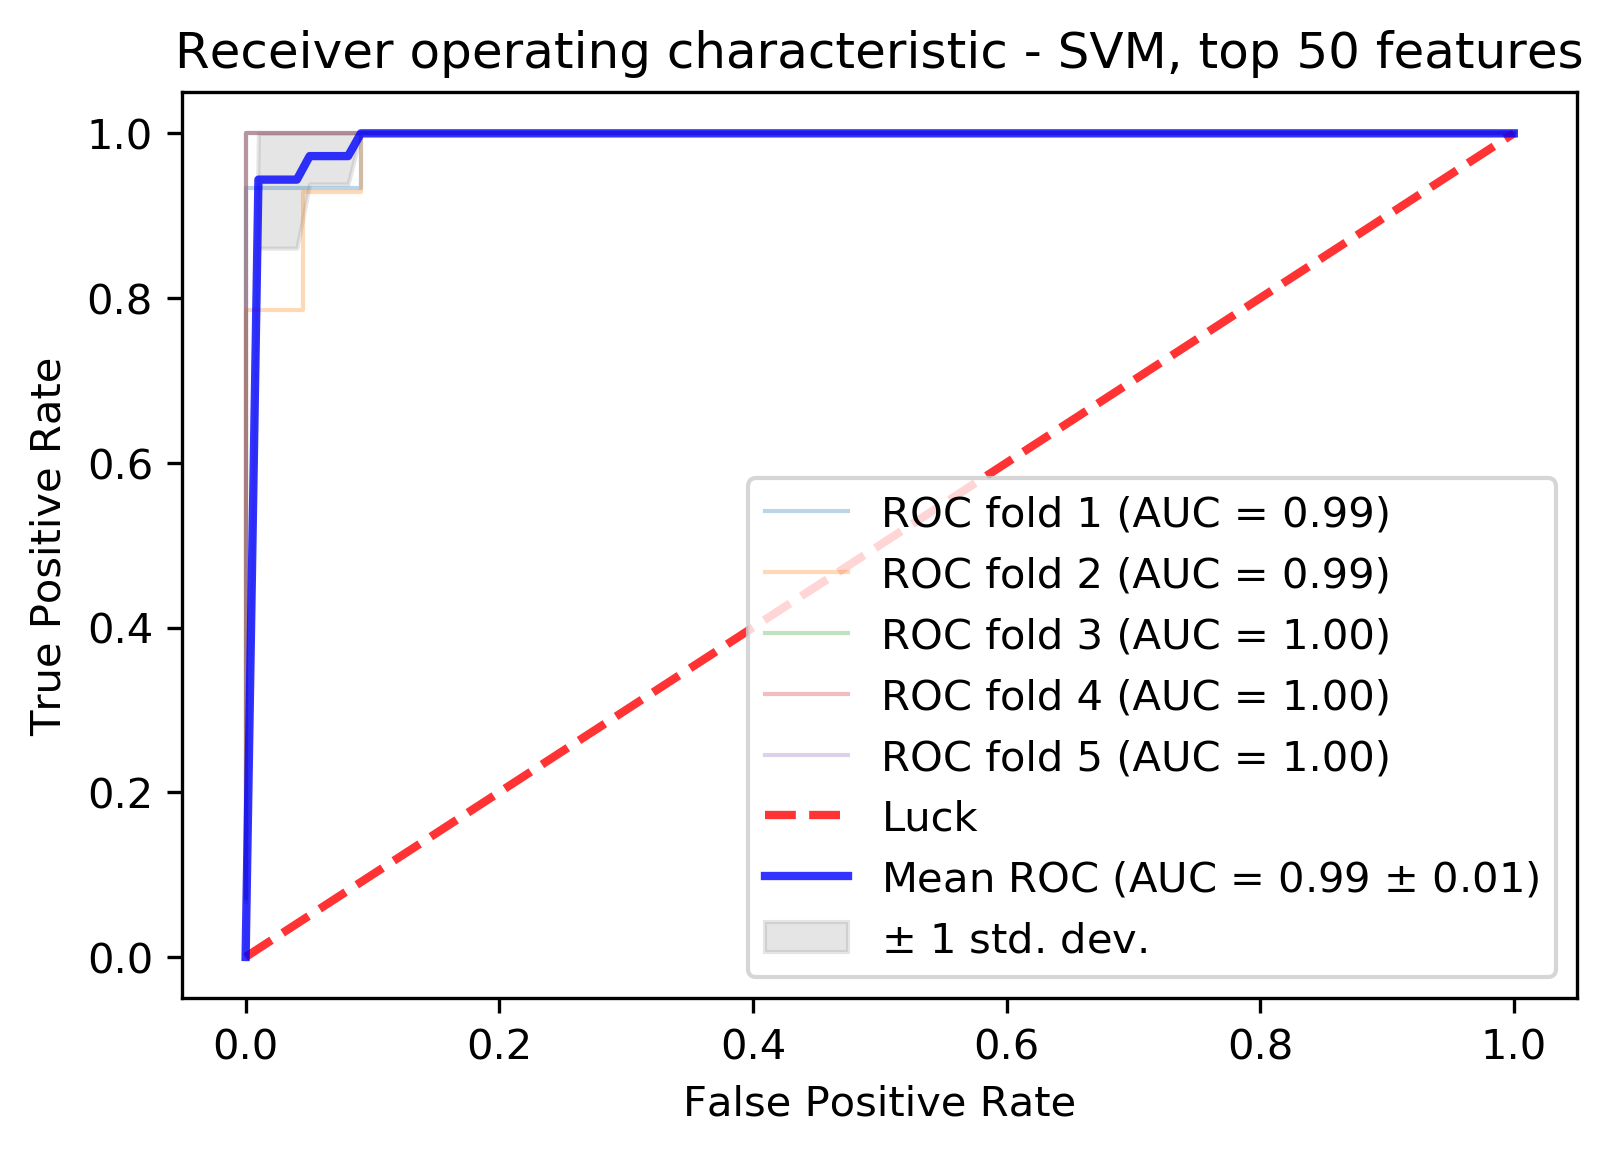
\includegraphics[width=5in]{../images/results/svm_top.png}
	\caption{ROC curve for the dataset with the top fifty features, with the Extra Trees Classifier.} 
	\label{fig:svm_top}
\end{figure}

